\documentclass[a4paper,11pt,fleqn]{article}
\usepackage[utf8]{inputenc}
\usepackage{natbib}
\usepackage{graphicx}
\usepackage{amsmath}
\usepackage{geometry}
\usepackage{booktabs}
\geometry{left=2.0cm, right=2.0cm, top=4.0cm, bottom=2.0cm}

\title{B1 Probability Theory and Statistical Inference Computer Assignment : Continuous Random Variables}
\author{Jiayue Zeng }
\date{September 2016}

\begin{document}

\maketitle

\section{Assignment 1 (Theoretical distributions)}
\subsection{Distributions and parameters}
Because the random sample of n independent observations $\; X_i$, $  i=1,2,...,n $ are from a population that follows a  $N(\mu,\sigma^2)$ distribution, where $\mu = 0 $ 
and $ \sigma^2 = 1$. 
So that the distribution of $\;Z_1, Z_2, Z_3, Z_4, and \;Z_5 $ are:
\vskip 0.5cm
According to THEOREM 7.1 (pg.353, Wackerly, endenhall, and Scheaffer) , we can know that, $Z_1$ is normally distributed with mean $\mu_{Z1}=0$ and variance $\sigma^2_{Z1}=\frac{1}{n}$ .
\vskip 0.5cm
$Z_1 = \overline{X} 
\sim N(0,\frac{1}{n}) $

\vskip 0.5cm
According to THEOREM 7.3 (pg.357, Wackerly, endenhall, and Scheaffer) , we can know that, $Z_2$ has a $\chi^2$ distribution with (n-1) degrees of freedom (df).

\vskip 0.5cm
$
Z_2 = \frac{\sum_{i=1}^{n}(X_{i}-\overline{X})^2}{\sigma^2}
\sim \chi^2(n-1)
$
\vskip 0.5cm
According to THEOREM 7.2 (pg.356, Wackerly, endenhall, and Scheaffer) , we can know that, $Z_3$ has a $\chi^2$ distribution with n degrees of freedom (df).
\vskip 0.5cm
$
Z_3 = \frac{\sum_{i=1}^{n}(X_i-\mu)^2}{\sigma^2}
\sim \chi^2(n) 
$
\vskip 0.5cm
Notice that the top part of the equation is the same equation as the normal distribution equation($Z_1$), and the lower part of the equation is a $\chi^2$ distribution. According to DEFINITION 7.2 (pg.360, Wackerly, endenhall, and Scheaffer) , we can know that, $Z_4$ has a t distribution with (n-1) degrees of freedom (df).
\vskip 0.5cm
$
Z_4 = \frac{\frac{\overline{X}-\mu}{\sigma/\sqrt{n}}}{\sqrt{\frac{\sum_{i=1}^{n}(X_i-\overline{X})^2}{(n-1)\sigma^2}}}
\sim  t(n-1)
$
\vskip 0.5cm
Notice that the top part and the lower part of the equation are independent $\chi^2$ distributed random variables with n and m df, respectively. According to DEFINITION 7.3 (pg.362, Wackerly, endenhall, and Scheaffer) , we can know that, $Z_5$ has an F distribution with n numerator degrees of freedom and m denominator degrees of freedom.
\vskip 0.5cm
$
Z_5 = \frac{\frac{\sum_{i=1}^{n}(X_i-\overline{X})^2}{(n-1)\sigma^2}}{\frac{\sum_{i=1}^{n}(Y_i-\overline{Y})^2}{(m-1)\sigma^2}}
\sim F(n-1,m-1) 
$
\vskip 0.7cm


\subsection{Formula of the expected value, variance, and standard deviation}
According to 1.1, we can know that the formulas for the statistic’s expected value, variance, its standard deviation are:
\vskip 0.5cm
$E(Z_1) = \mu = 0 \;\;
Var(Z_1) = \frac{\sigma^2}{n} = \frac{1}{n}   \;\;\;\;
sd(Z_1) = \frac{\sigma}{\sqrt{n}} = \frac{1}{\sqrt{n}}
$
\vskip 0.5cm
$E(Z_2) = n-1  \;\;
Var(Z_2) = 2(n-1)  \;\;\;
sd(Z_2) = \sqrt{2(n-1)}  \;\;
$
\vskip 0.5cm
$E(Z_3) = n  \;\qquad
Var(Z_3) = 2n  \;\;\;\;\;\qquad
sd(Z_3) = \sqrt{2n} 
$
\vskip 0.5cm
$E(Z_4) = 0 \;\;\qquad
Var(Z_4) = \frac{n}{n-2}\;\;\;\qquad
sd(Z_4) = \sqrt{\frac{n}{n-2}}
$
\vskip 0.5cm
$E(Z_5) = \frac{m-1}{m-3}\;\quad
Var(Z_5) = \frac{2(m-1)^2(m+n-4)}{(n-1)(m-3)^2(m-5)}\;\;
sd(Z_5) = \sqrt{\frac{2(m-1)^2(m+n-4)}{(n-1)(m-3)^2(m-5)}}\;\;
$


\vskip 0.7cm
\subsection{Table of the five statistics}


When $n = 5$, the expected value, variance, and standard deviation for the statistics $Z_1$ to $Z_4$ are listed in Table 1. 

\vskip 0.5cm

\begin{table}[htbp]
\caption{The expected value, variance, and standard deviation of $\;Z_1, Z_2, Z_3, Z_4 $}
\vskip 0.5cm
\centering
 \begin{tabular}{lclclclclcl}
  \toprule
statistic &$Z_1$  &$Z_2$  &$Z_3$  &$Z_4$  \\
  \midrule
$E$       & 0.000  &  4.000 & 5.000    & 0.000 \\
$Var$     & 0.200   &  8.000    & 10.000   & 2.000 \\
$sd $     & 0.447  &  2.828 & 3.162 & 1.414\\
  \bottomrule
 \end{tabular}
\end{table}

\vskip 0.5cm
When $n = 20$, the expected value, variance, and standard deviation for the statistics $Z_1$ to $Z_4$ are listed in Table 2. 

\begin{table}[htbp]
\caption{The expected value, variance, and standard deviation of $\;Z_1, Z_2, Z_3, Z_4 $}
\vskip 0.5cm
\centering
 \begin{tabular}{lclclclclcl}
  \toprule
statistic &$Z_1$  &$Z_2$  &$Z_3$  &$Z_4$  \\
  \midrule
$E$       & 0.000     &  19.000    & 20.000    & 0.000 \\
$Var$     & 0.050  &  38.000    & 40.000    & 1.118 \\
$sd $     & 0.224  &  6.164  & 6.325   & 1.057\\
  \bottomrule
 \end{tabular}
\end{table}



\vskip 0.5cm
When $n = 5,\; m = 20 $, the expected value, variance, and standard deviation for the statistics $Z_1$ to $Z_4$ are listed in Table 3. 

\begin{table}[htbp]
\caption{The expected value, variance, and standard deviation of $\;Z_5 $}
\vskip 0.5cm
\centering
 \begin{tabular}{lclclclclcl}
  \toprule
statistic &$Z_5$   \\
  \midrule
$E$       & 1.118   \\
$Var$     & 0.874   \\
$sd $     & 0.935   \\
  \bottomrule
 \end{tabular}
\end{table}




\section{Assignment 2 (Empirical distributions)}
\subsection{Statistics $Z_1, Z_2, Z_3$ and $Z_4$}
Draw 1000 samples of size n = 5 and n = 20 from the population. Based on these samples, evaluate all four statistics.
\vskip 0.5cm

When $n = 5$,  the mean, variance, and standard deviation of the 1000 samples the for the statistics $Z_1$ to $Z_4$ are listed in Table 4.  According to the Table 4, for each of the four statistics, the mean, variance, and standard deviation of the 1000 samples are approximately equal to  the theoretical values.

\vskip 0.5cm

\begin{table}[htbp]
\caption{The mean, variance, and standard deviation of $\;Z_1, Z_2, Z_3, Z_4 $}
\vskip 0.5cm
\centering
 \begin{tabular}{lclclclclcl}
  \toprule
Empirical &$Z_1$  &$Z_2$  &$Z_3$  &$Z_4$ \\
  \midrule
$mean$   & -0.004 &  4.191    & 5.272    & -0.005 \\
$Var$     & 0.215   &  8.375    & 10.379 & 2.229  \\
$sd $     & 0.464  &  2.894   & 3.222    & 1.493  \\
  \midrule
Theoretical &$Z_1$  &$Z_2$  &$Z_3$  &$Z_4$  \\
  \midrule
$E$       & 0.000  &  4.000 & 5.000    & 0.000 \\
$Var$     & 0.200   &  8.000    & 10.000   & 2.000 \\
$sd $     & 0.447  &  2.828 & 3.162 & 1.414\\
  \bottomrule
 \end{tabular}
\end{table}


\vskip 0.5cm

For each statistic, illustrate graphically the distribution of the 1000 values and compare with a graph for the theoretical distribution. The graphs are shown below.
\vskip 0.5cm
\begin{figure}[h!]
\centering
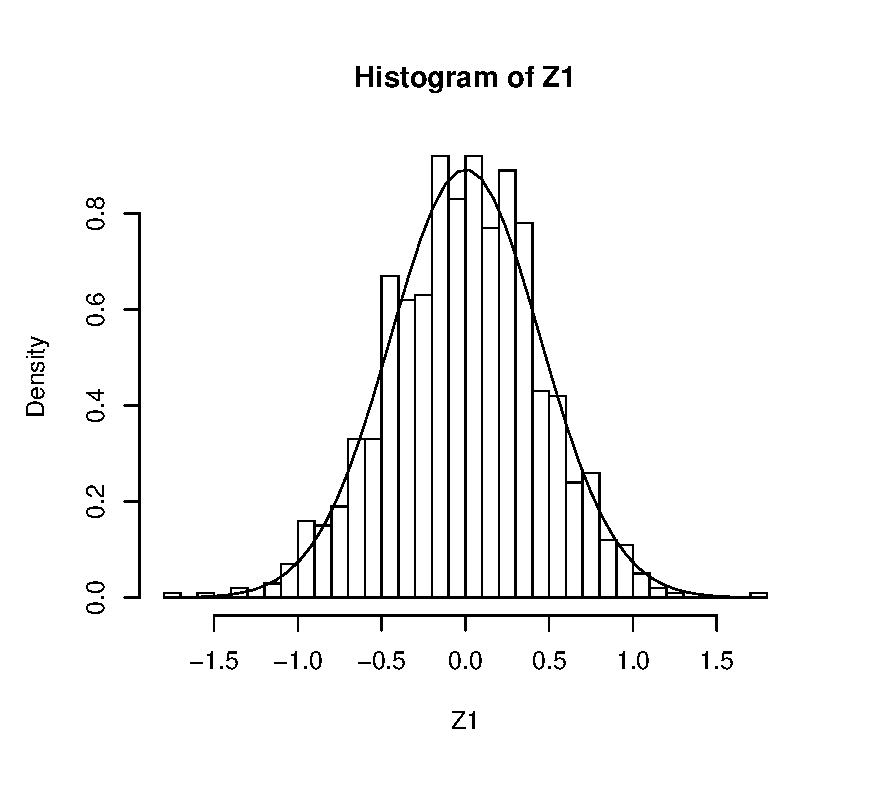
\includegraphics[scale=0.8]{Z1.eps}
\caption{Graph of $Z_1$}
\label{fig: $Z_1$}
\end{figure}
\vskip 0.5cm

\begin{figure}[h!]
\centering
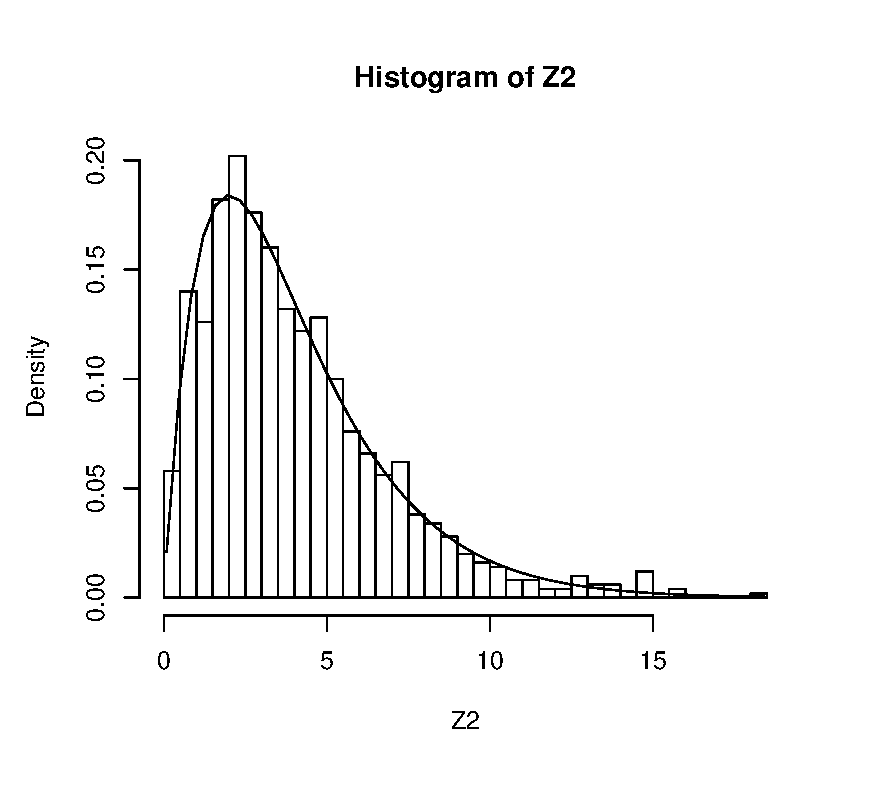
\includegraphics[scale=0.8]{Z2.eps}
\caption{Graph of $Z_2$}
\label{fig: $Z_2$}
\end{figure}
\vskip 0.5cm

\begin{figure}[h!]
\centering
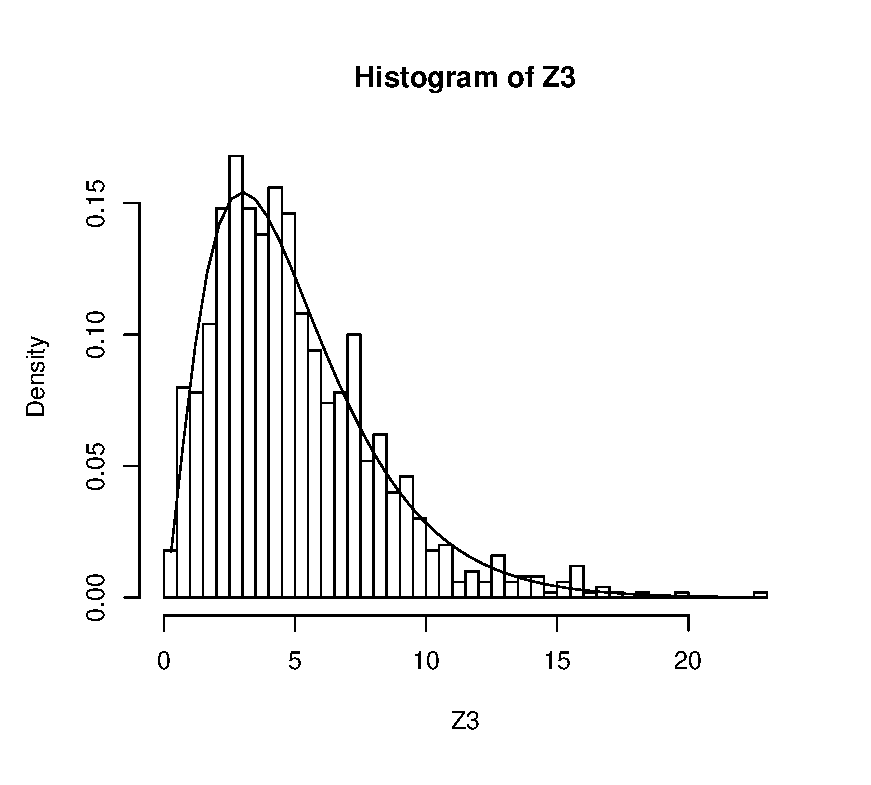
\includegraphics[scale=0.8]{Z3.eps}
\caption{Graph of $Z_3$}
\label{fig: $Z_3$}
\end{figure}
\vskip 0.5cm

\begin{figure}[h!]
\centering
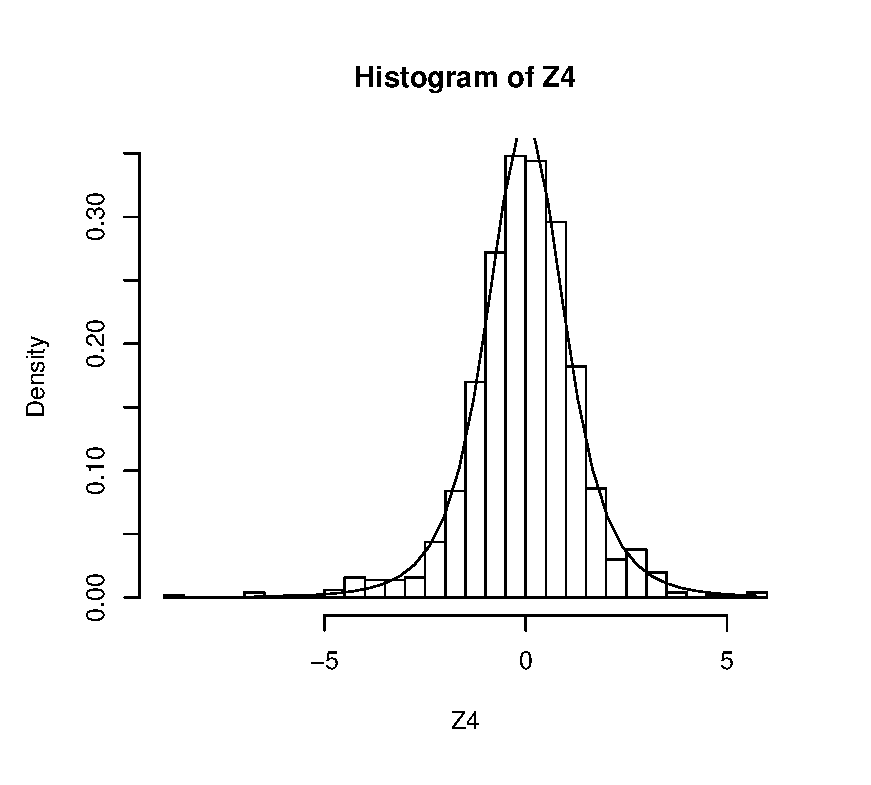
\includegraphics[scale=0.8]{Z4.eps}
\caption{Graph of $Z_4$}
\label{fig: $Z_4$}
\end{figure}



\vskip 0.5cm
\newpage
As the graphs show, the empirical distribution of $Z_1$ basically fits the theoretical distribution, a normal distribution where the expected value is 0 and the variance is $\frac{1}{5}$, with a certain amount of error.

The empirical distribution of $Z_2$ basically fits the theoretical distribution, a chi-square distribution where the degree of freedom is 4, with a certain amount of error.

The empirical distribution of $Z_3$ basically fits the theoretical distribution, a chi-square distribution where the degree of freedom is 5, with a certain amount of error.

The empirical distribution of $Z_4$ basically fits the theoretical distribution, a t-distribution where the parameter is 4, with a certain amount of error.

The reason why we can see that the empirical distributions do not fit the theoretical distribution really well is that the samples are random and the samples size is not big enough. If we increase the number of samples, the result will fit better.
\vskip 0.5cm
\newpage



When $n = 20$,  the mean, variance, and standard deviation of the 1000 samples the for the statistics $Z_1$ to $Z_4$ are listed in Table 5. According to the Table 5, for each of the four statistics, the mean, variance, and standard deviation of the 1000 samples are approximately equal to  the theoretical values.
\vskip 0.5cm

\begin{table}[htbp]
\caption{The mean, variance, and standard deviation of $\;Z_1, Z_2, Z_3, Z_4 $}
\vskip 0.5cm
\centering
 \begin{tabular}{lclclclclcl}
 \toprule
Empirical &$Z_1$  &$Z_2$  &$Z_3$  &$Z_4$  \\
 \midrule
$mean$    & -0.009   &  19.225   & 20.211    & -0.045 \\
$Var$     & 0.0484   &  38.415   & 41.190    & 1.055 \\
$sd $     & 0.220    &  6.198    & 6.418     & 1.027 \\
 \midrule
Theoretical &$Z_1$  &$Z_2$  &$Z_3$  &$Z_4$  \\
  \midrule
$E$       & 0.000     &  19.000    & 20.000    & 0.000 \\
$Var$     & 0.050  &  38.000    & 40.000    & 1.118 \\
$sd $     & 0.224  &  6.164  & 6.325   & 1.057\\
  \bottomrule
 \end{tabular}
\end{table}


\vskip 0.5cm
For each statistic, illustrate graphically the distribution of the 1000 values and compare with a graph for the theoretical distribution. The graphs are shown below.
\vskip 0.5cm
\begin{figure}[h!]
\centering
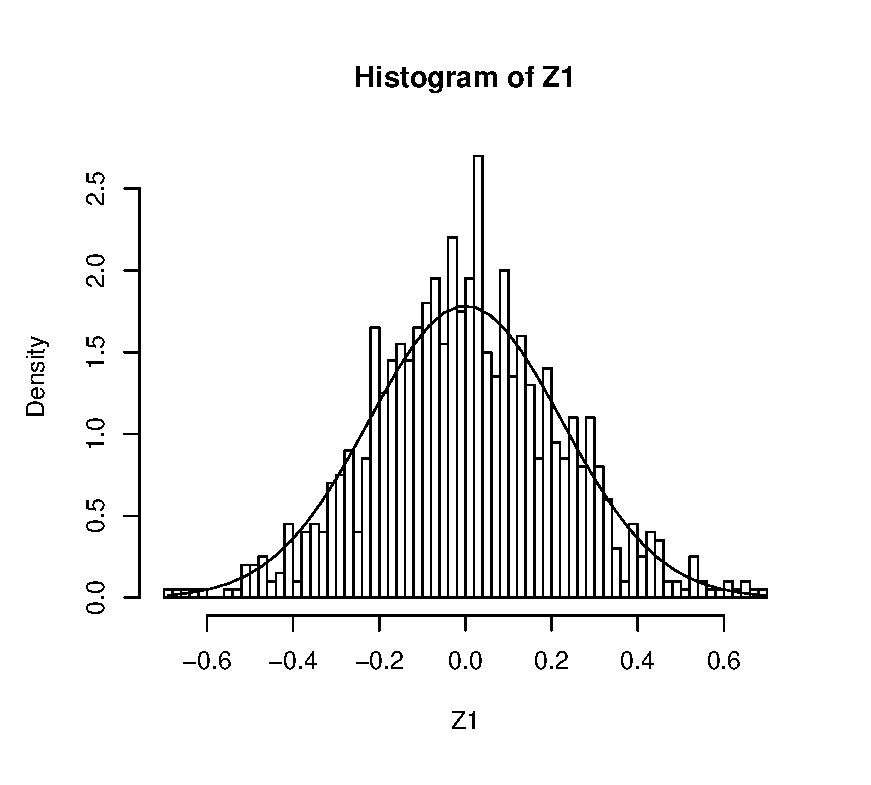
\includegraphics[scale=0.8]{Z120.eps}
\caption{Graph of $Z_1$}
\label{fig: $Z_1$}
\end{figure}
\vskip 0.5cm


\begin{figure}[h!]
\centering
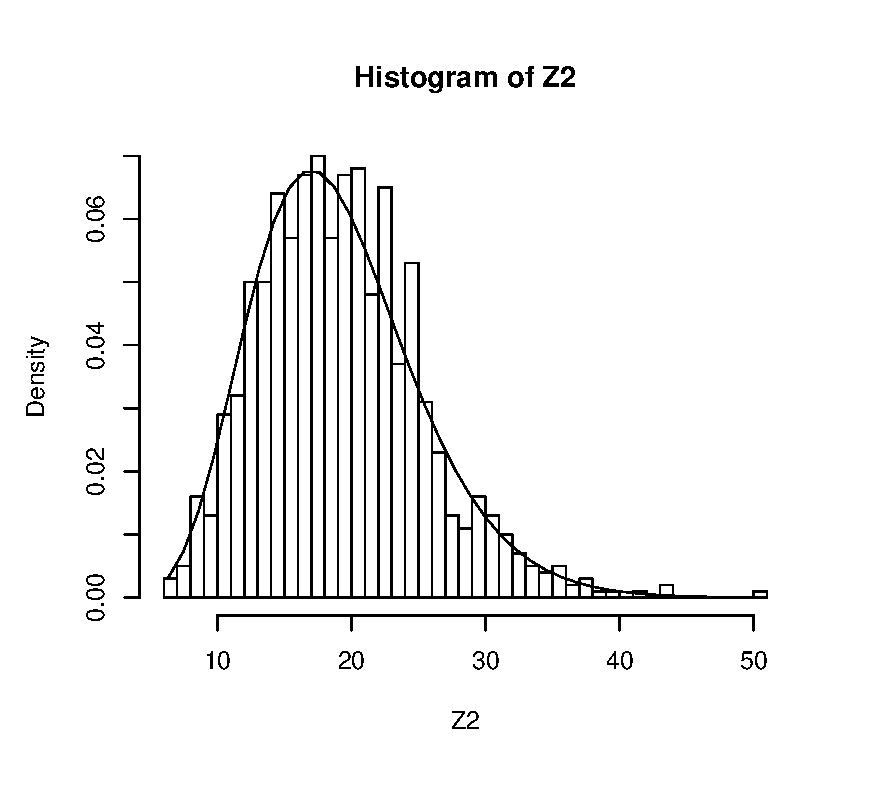
\includegraphics[scale=0.8]{Z220.eps}
\caption{Graph of $Z_2$}
\label{fig: $Z_2$}
\end{figure}
\vskip 0.5cm

\begin{figure}[h!]
\centering
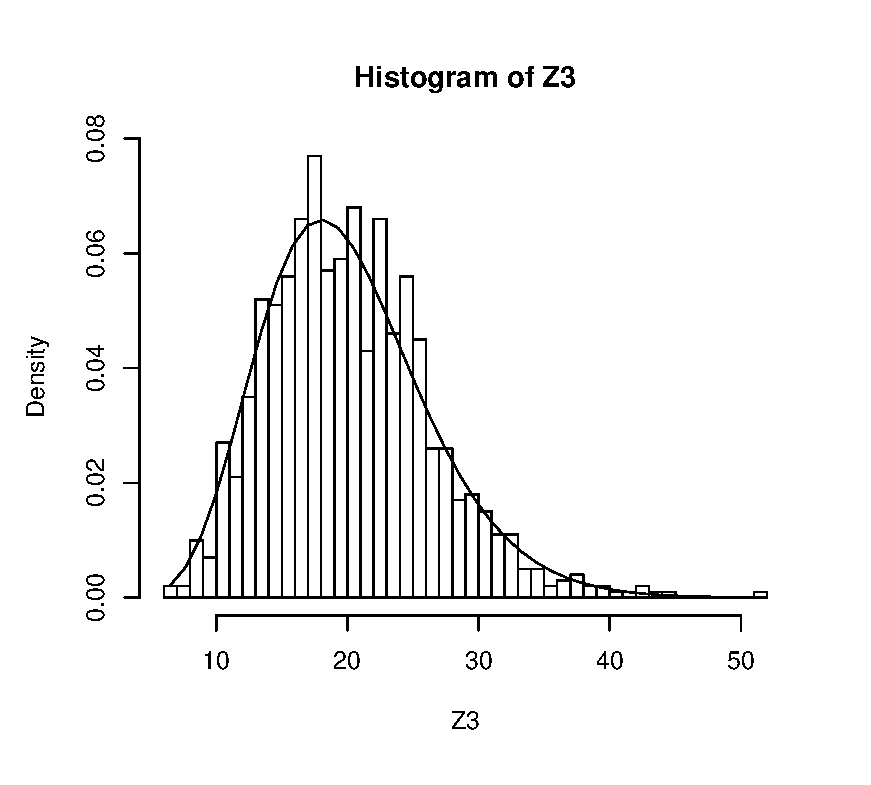
\includegraphics[scale=0.8]{Z320.eps}
\caption{Graph of $Z_3$}
\label{fig: $Z_3$}
\end{figure}
\vskip 0.5cm

\begin{figure}[h!]
\centering
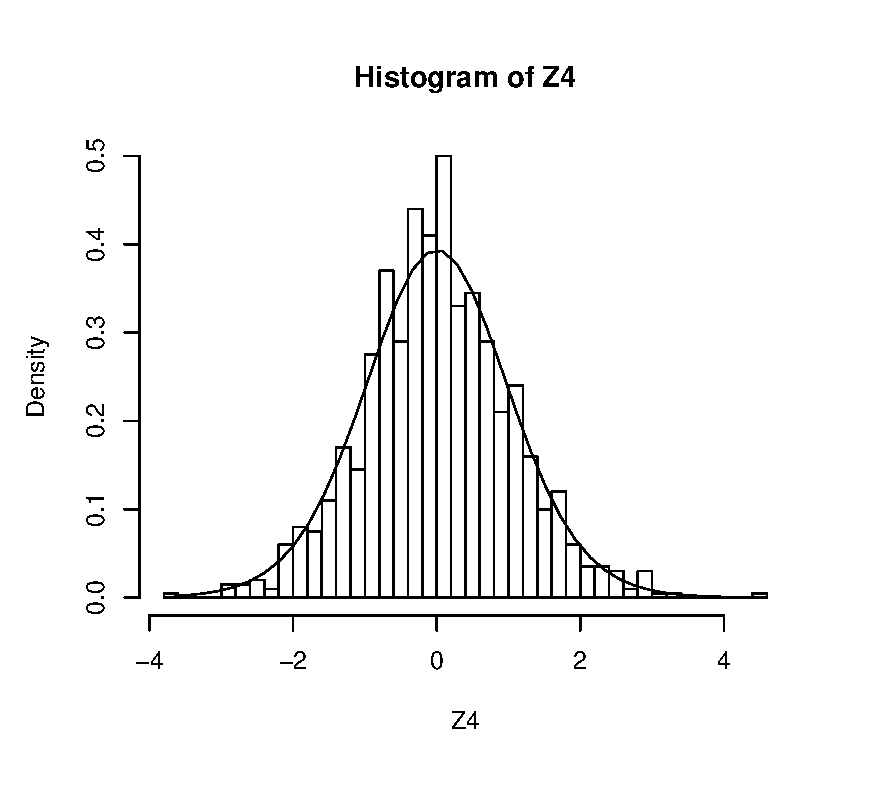
\includegraphics[scale=0.8]{Z4_20.eps}
\caption{Graph of $Z_4$}
\label{fig: $Z_4$}
\end{figure}


\vskip 0.5cm

As the graphs show, the empirical distribution of $Z_1$ basically fits the theoretical distribution, a normal distribution where the expected value is 0 and the variance is $\frac{1}{20}$, with a certain amount of error.

The empirical distribution of $Z_2$ basically fits the theoretical distribution, a chi-square distribution where the degree of freedom is 19, with a certain amount of error.

The empirical distribution of $Z_3$ basically fits the theoretical distribution, a chi-square distribution where the degree of freedom is 20, with a certain amount of error.

The empirical distribution of $Z_4$ basically fits the theoretical distribution, a t-distribution where the parameter is 19, with a certain amount of error.

The reason why we can see that the empirical distributions do not fit the theoretical distribution really well is that the samples are random and the samples size is not big enough. If we increase the number of samples, the result will fit better.
\vskip 0.5cm
\vskip 0.5cm


\newpage
\subsection{Statistic $Z_5$ }
\vskip 0.5cm
When $n = 5, \;m = 20$, When $n = 5$,  the mean, variance, and standard deviation of the 1000 samples for the statistics $Z_1$ to $Z_4$ are listed in Table 6. According to the Table 6, the mean, variance, and standard deviation of $Z_5$ are approximately equal to  the theoretical values.

\vskip 0.5cm

\begin{table}[htbp]
\caption{The mean, variance, and standard deviation of $\;Z_5 $}
\vskip 0.5cm
\centering
 \begin{tabular}{lclclclclcl}
 \toprule
Empirical &$Z_5$  & Theoretical &$Z_5$\\
 \midrule
$mean$    & 1.097 &$E$       & 1.118 \\
$Var$     & 0.920 &$Var$     & 0.874\\
$sd $     & 0.959 &$sd $     & 0.935  \\

  \bottomrule
 \end{tabular}
\end{table}

\begin{figure}[h!]
\centering
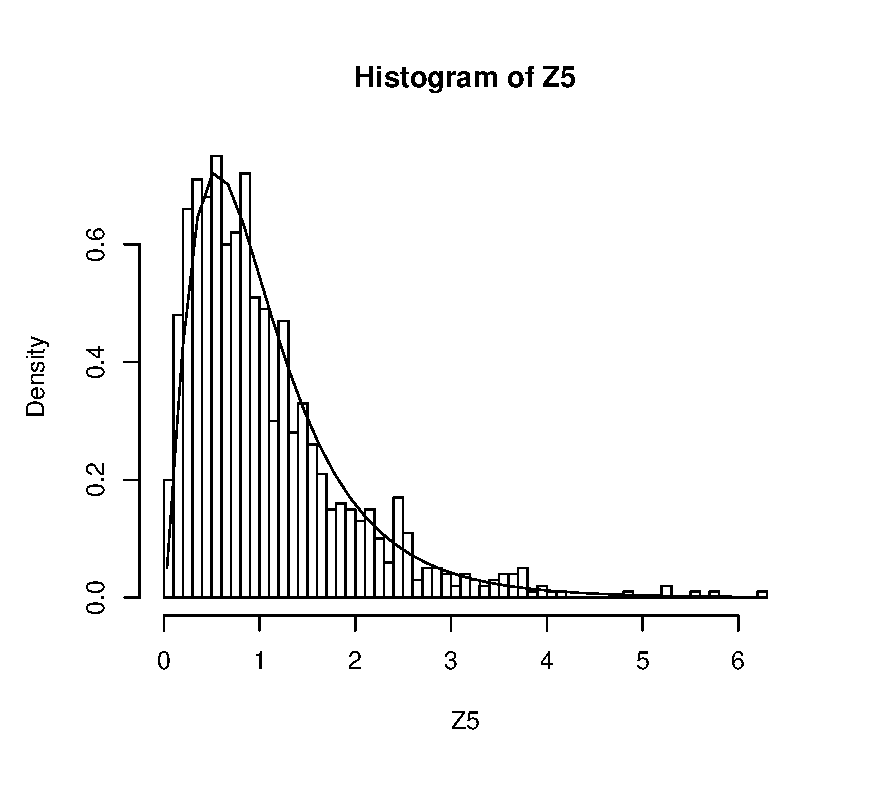
\includegraphics[scale=0.8]{Z5.eps}
\caption{Graph of $Z_5$}
\label{fig: $Z_5$}
\end{figure}

As the graph shows, the empirical distribution of $Z_5$ basically fits the theoretical distribution, an F-distribution where the parameters are 5 and 20, with a certain amount of error.The reason why we can see that the empirical distributions do not fit the theoretical distribution really well is that the samples are random and the samples size is not big enough. If we increase the number of samples, the result will fit better.


\end{document}
